\section{Funktionen}\label{sec:Die Funktion}
Eine Funktion ist eine Zuordnung aus zwei Zahlenmengen. Die Funktion $f:D\rightarrow \mathbb{R}$ mit $D\in \mathbb{R}$. Sei $a\in X$ und $b\in Y$, so bildet $a\mapsto b$ ab, und stellt somit ein Zuordnung zweier Mengen dar. Hierbei wird jedem $x$ ein $y$ zu. 
%ToDo Die Definition sollte hier nochmals überarbeitet werden

\begin{beispiel} Fährt man mit einem Auto konstant 100km/h, so kann man dies auch in einer Wertetabelle darstellen. Hierbei ist zu beachten, dass die Funktion Kilometer in Zeit darstellt.
\begin{align*}
	1 \text{ Stunde}&\mapsto100 \text{ Kilometer}\\
	2 \text{ Stunde}&\mapsto200 \text{ Kilometer}\\
	3 \text{ Stunde}&\mapsto300 \text{ Kilometer}\\
	4 \text{ Stunde}&\mapsto400 \text{ Kilometer}
\end{align*}
\end{beispiel}
\subsection{Darstellung von Funktionen}\label{sec:Die Funktion/Darstellen von Funktionen}
Setzt man in eine Funktion für das $x$ einen Wert, so erhält man den zugehörigen $y$-Wert. Dieses Wertepaar lässt sich in ein Koordinatensystem eintragen (\ref{sec:Wertetabelle_einer_Funktion_visualisiert}). Verbindet man nun die Punkte miteinand er, so entsteht der sogenannte Funktionsgraph. Auch lässt sich hierbei leicht erkennen, ob es sich überhaupt um eine Funktion, handelt. Betrachtet man die $Y$-Achse, als den obig erwähnten Wert und die $X$-Achse als Ausgangsmenge, so lässt sich feststellen, warum eine Funktion keine Zuweisung von zwei $X$-Werten haben kann.
%ToDo Warum hatt eine Funktion keine zwei X-Werte
\begin{figure}[h!]
\centering
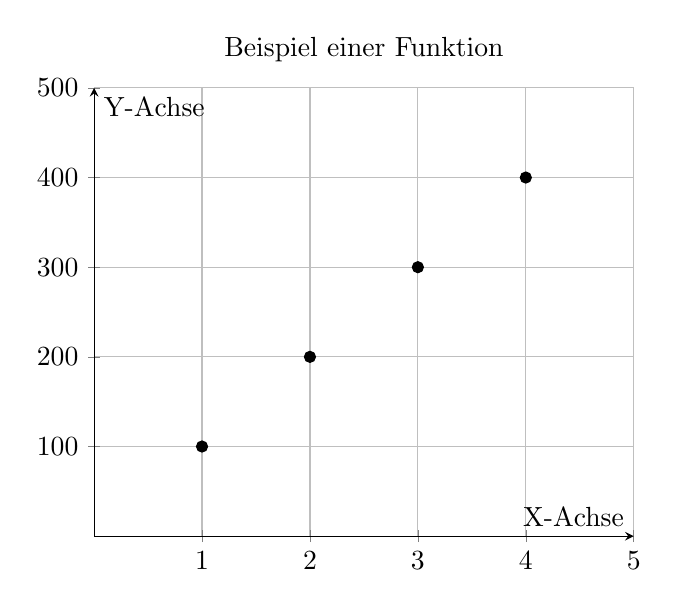
\begin{tikzpicture}
\begin{axis}[
    title={Beispiel einer Funktion},
    xlabel={X-Achse},
    ylabel={Y-Achse},
    axis lines=middle, % Zentriert die Achsen
    xmin=0, xmax=5, % Setzt die Grenzen für die X-Achse
    ymin=0, ymax=500, % Setzt die Grenzen für die Y-Achse
    grid=major, % Fügt ein Hauptgitter hinzu
]
\addplot[mark=*] coordinates {(1,100)};
\addplot[mark=*] coordinates {(2,200)};
\addplot[mark=*] coordinates {(3,300)};
\addplot[mark=*] coordinates {(4,400)};
\end{axis}
\end{tikzpicture}
\caption{Wertetabelle einer Funktion visualisiert}
\label{sec:Wertetabelle_einer_Funktion_visualisiert}
\end{figure}

 
